\section{Dataset}
\label{sec:Dataset}

To train a machine learning model and achieve reasonable good results, a good data base is needed. For getting accurate market price predictions
for motorcycles, one needs up to date market data of motorcycles. This is given by the dataset \textit{"USA Comprehensive Motorcycles Dataset 9k+"}\cite{kaggle_1}
and \textit{"Motorcycle Specifications Dataset"}\cite{kaggle_2}, which both can be found on \textbf{kaggle.com} and underly a \textit{CC0:Public Domain} License.\\
The first dataset provides market prices, model, mileage and year of manifacture for the brands \textit{BMW}, \textit{KTM}, \textit{Royal Enfield}, \textit{Suzuki}, \textit{Yamaha} and \textit{Ducati}
up to 2023. Although only six different brands are provided, these already cover most of the current motorcycle market. The second dataset provides additional 
information for the single motorcycle models like displacement, power or the number of cylinders.

\subsection{Preprocessing}

A common first step for machine learning tasks is the preprocessing of the dataset. According to the quality of the dataset, this 
can be more or less tidious. As for the final dataset used in this report, this step took longer than hoped for. As the data for all brands
were provided seperately, as well as the dataset for the model specifications one of the major task was to merge the bike specification columns (displacement, ...)
to the datasets containing the prices. An excerpt of the used datesets is shown in \autoref{fig:Bike_Tables_raw}. An enlarged view on the
datasets is shown in the \autoref{sec:Appendix}.
\begin{figure}
    \centering
    \begin{subfigure}[h]{0.325\textwidth}
        \centering
        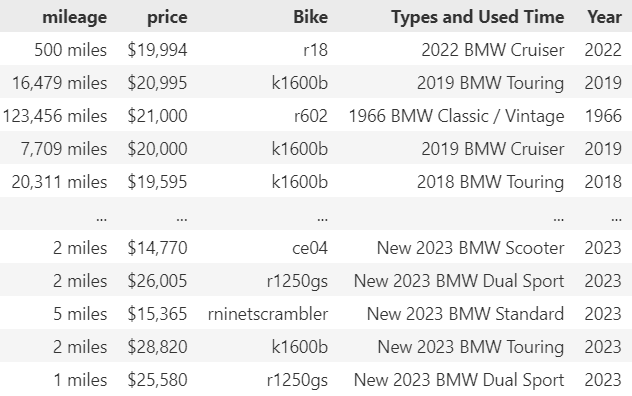
\includegraphics[width=\textwidth]{"content/pics/df_bmw_raw.png"}
    \end{subfigure}
    \hfill
    \begin{subfigure}[h]{0.66\textwidth}
        \centering
        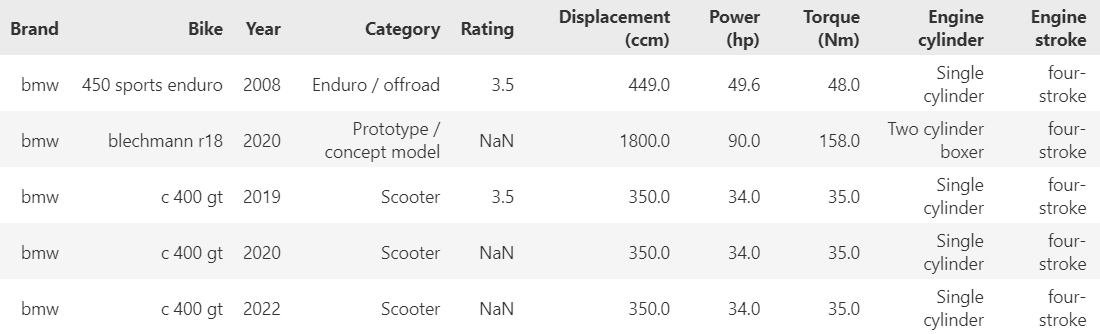
\includegraphics[width=\textwidth]{"content/pics/df_bikez_raw.png"}
    \end{subfigure}
    \caption{Excerpt of one of the datasets containing the price and selling specifications (left) and the dataset
    containing the motorcycle specifications (right).}
    \label{fig:Bike_Tables_raw}
\end{figure}
\\ Before merging the datasets, the columns have to be properly cleaned. For this purpose, a descriptional column of the datasets
containing the prices was discarded, as it does not give additional information in a uniform way. Some entries had information about
the bike condition or the limitation of the model in that column. Secondly, the year of manifacture was extracted from the \textit{Types and Used Time}
column and all entries with no information on the price and mileage were dropped. The \textit{Bike} column of the price datasets
and the \textit{Bike} column of the specifications dataset were brought to the same formatting and style, such that a merge between those
datasets is possible.\\
Finally, the datasets are merged, based on the bike model and the year of manifacture. For those cases, where there is no matching
bike model for the exact year of manifacture in the specifications dataset, the entries are merged with another year of manifacture 
of that exact model. Some bike models of the specifications dataset were missing some column entries like \textit{Category} for some years
of manifacture. These entries were filled with matching bike models, but different years of manifacture. It does happen, that some specifications
like power or displacement changes over the different years of manifacture slightly, but the used method should yield a very
good approximation of the real column entries. At this point, all entries for which the column \textit{Category} is empty, are dropped.\\
Next, NaN entries are filled with the mean value of the corresponding bike category, the \textit{mileage} and  \textit{price} column data types are fixed to 
be integers instead of strings and calculated into kilometres and euros instead of miles and dollars.\\
All brand subsets are concatenated
to form one big dataset and the final columns used for further analysis are chosen as \textit{Mileage [km], Price [€], Bike, 
Brand, Category, Displacement [ccm], Power [hp], Torque [Nm], Condition and Age [a]}.
The condition column contains boolean values for Used (\texttt{True}) and New (\texttt{False}) based on the mileage. The age is the 
relative used age of the motorcycle ($2023 - \mathrm{Year}$).

\subsection{Exploratory Data Analysis}
\label{sec:Expl}
Before throwing the dataset into some machine learning algorithms and hoping for good results, a logical approach is to look at 
the data distributions, correlations of the attributes with each other and the price and look for useful data scaling methods.
As some of the columns contain categorical data (like \textit{Bike}), they need to be transformed into numerical 
data, to make use of them in a plot. For the \textit{Bike} and \textit{Category} column, a frequency mapping was chosen, meaning
that the string values were matched with the frequency of that relative string. This is a common approach for categorical columns,
with a broad varity of entries. For the \textit{Brand} column, a dummy column is created. This means,
that for each unique value of the respective column, a new column with boolean values is created. \\
To get a general understanding of the data distributions, a scatter matrix containing all columns (except the dummy columns) 
is presented in \autoref{fig:Scatterplot_All}.
\begin{figure}[h]
    \centering
        \makebox[\textwidth][h]{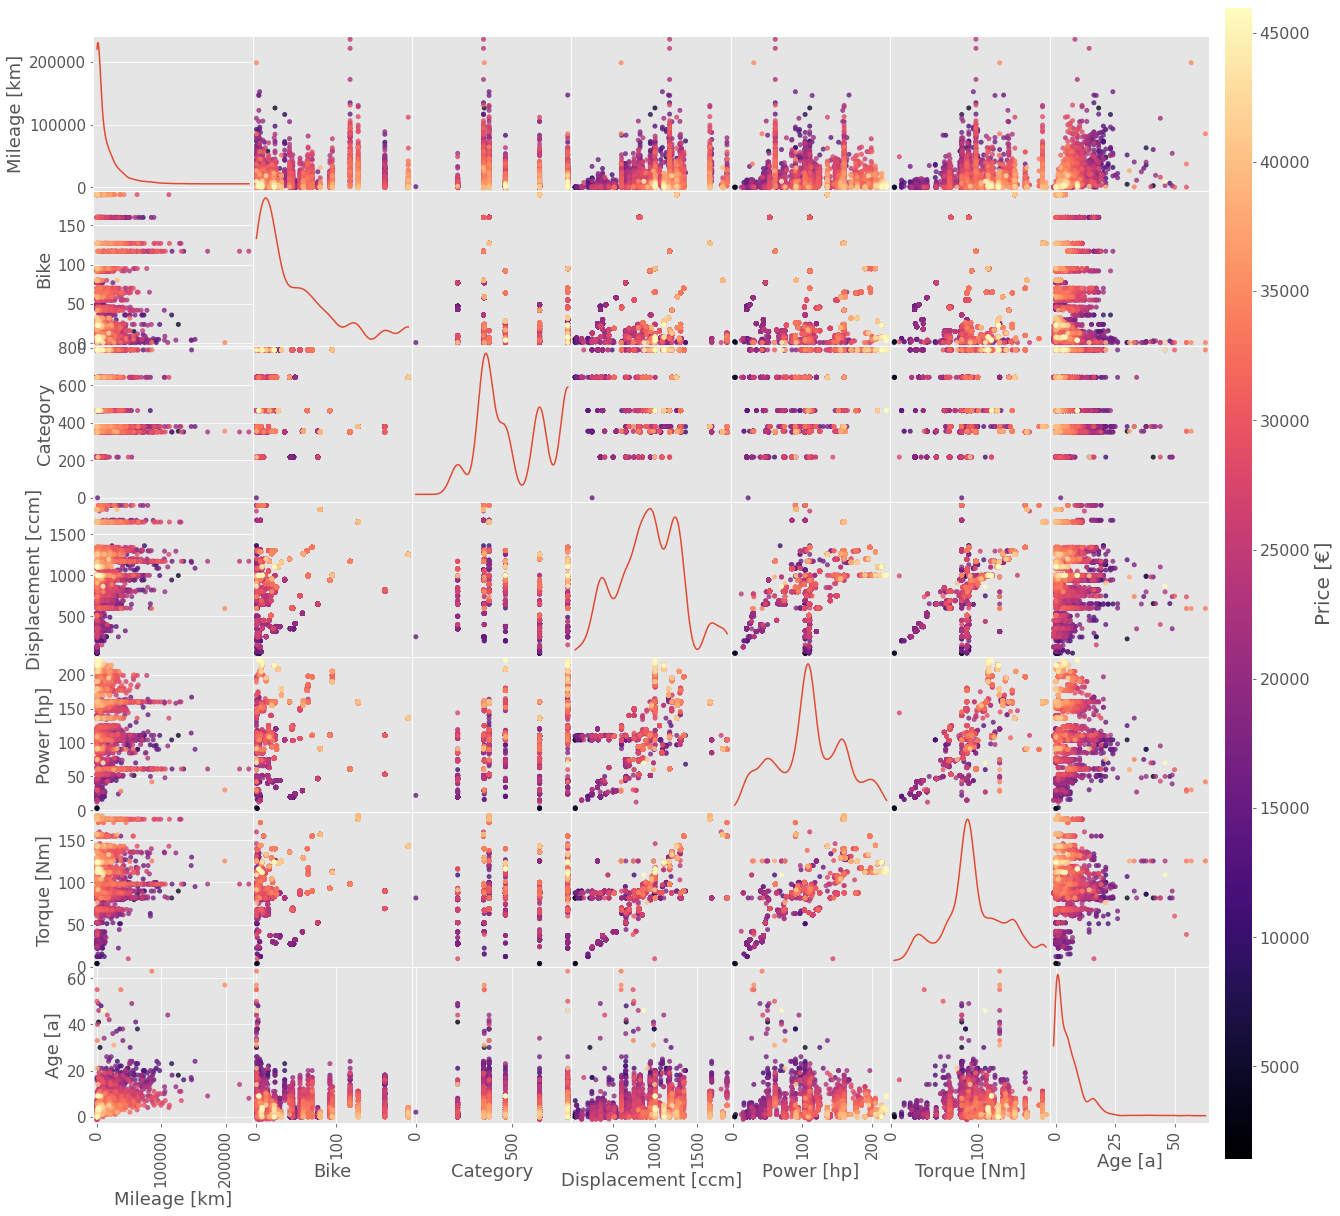
\includegraphics[width=0.9\textwidth]{"content/pics/Scatter_Matrix_All.png"}}
        \caption{Scatter matrix of all dataset columns (except dummy columns).}
        \label{fig:Scatterplot_All}
\end{figure}
It shows, that there are in general many newer motorcycles with a low age amount and little amount of mileage. The displacement,
power and torque are more or less normal distributed, with significant peaks in the mean value, which is due to the filling of \texttt{NaN}
values with the mean. Many scatter plox show already significant correlations, like the \textit{Power [hp]} - \textit{Torque [Nm]} (which
is very much expected as these two metrics are causally linked). The \autoref{fig:Scatterplot_Price} also shows clear dependencies
of the price on the used attributes, making them useful for regression problems. Motorcycles with a low \textit{age} and \textit{mileage} and a high amount
of \textit{power} should yield the highest prices.
\begin{figure}
    \centering
        \makebox[\textwidth][h]{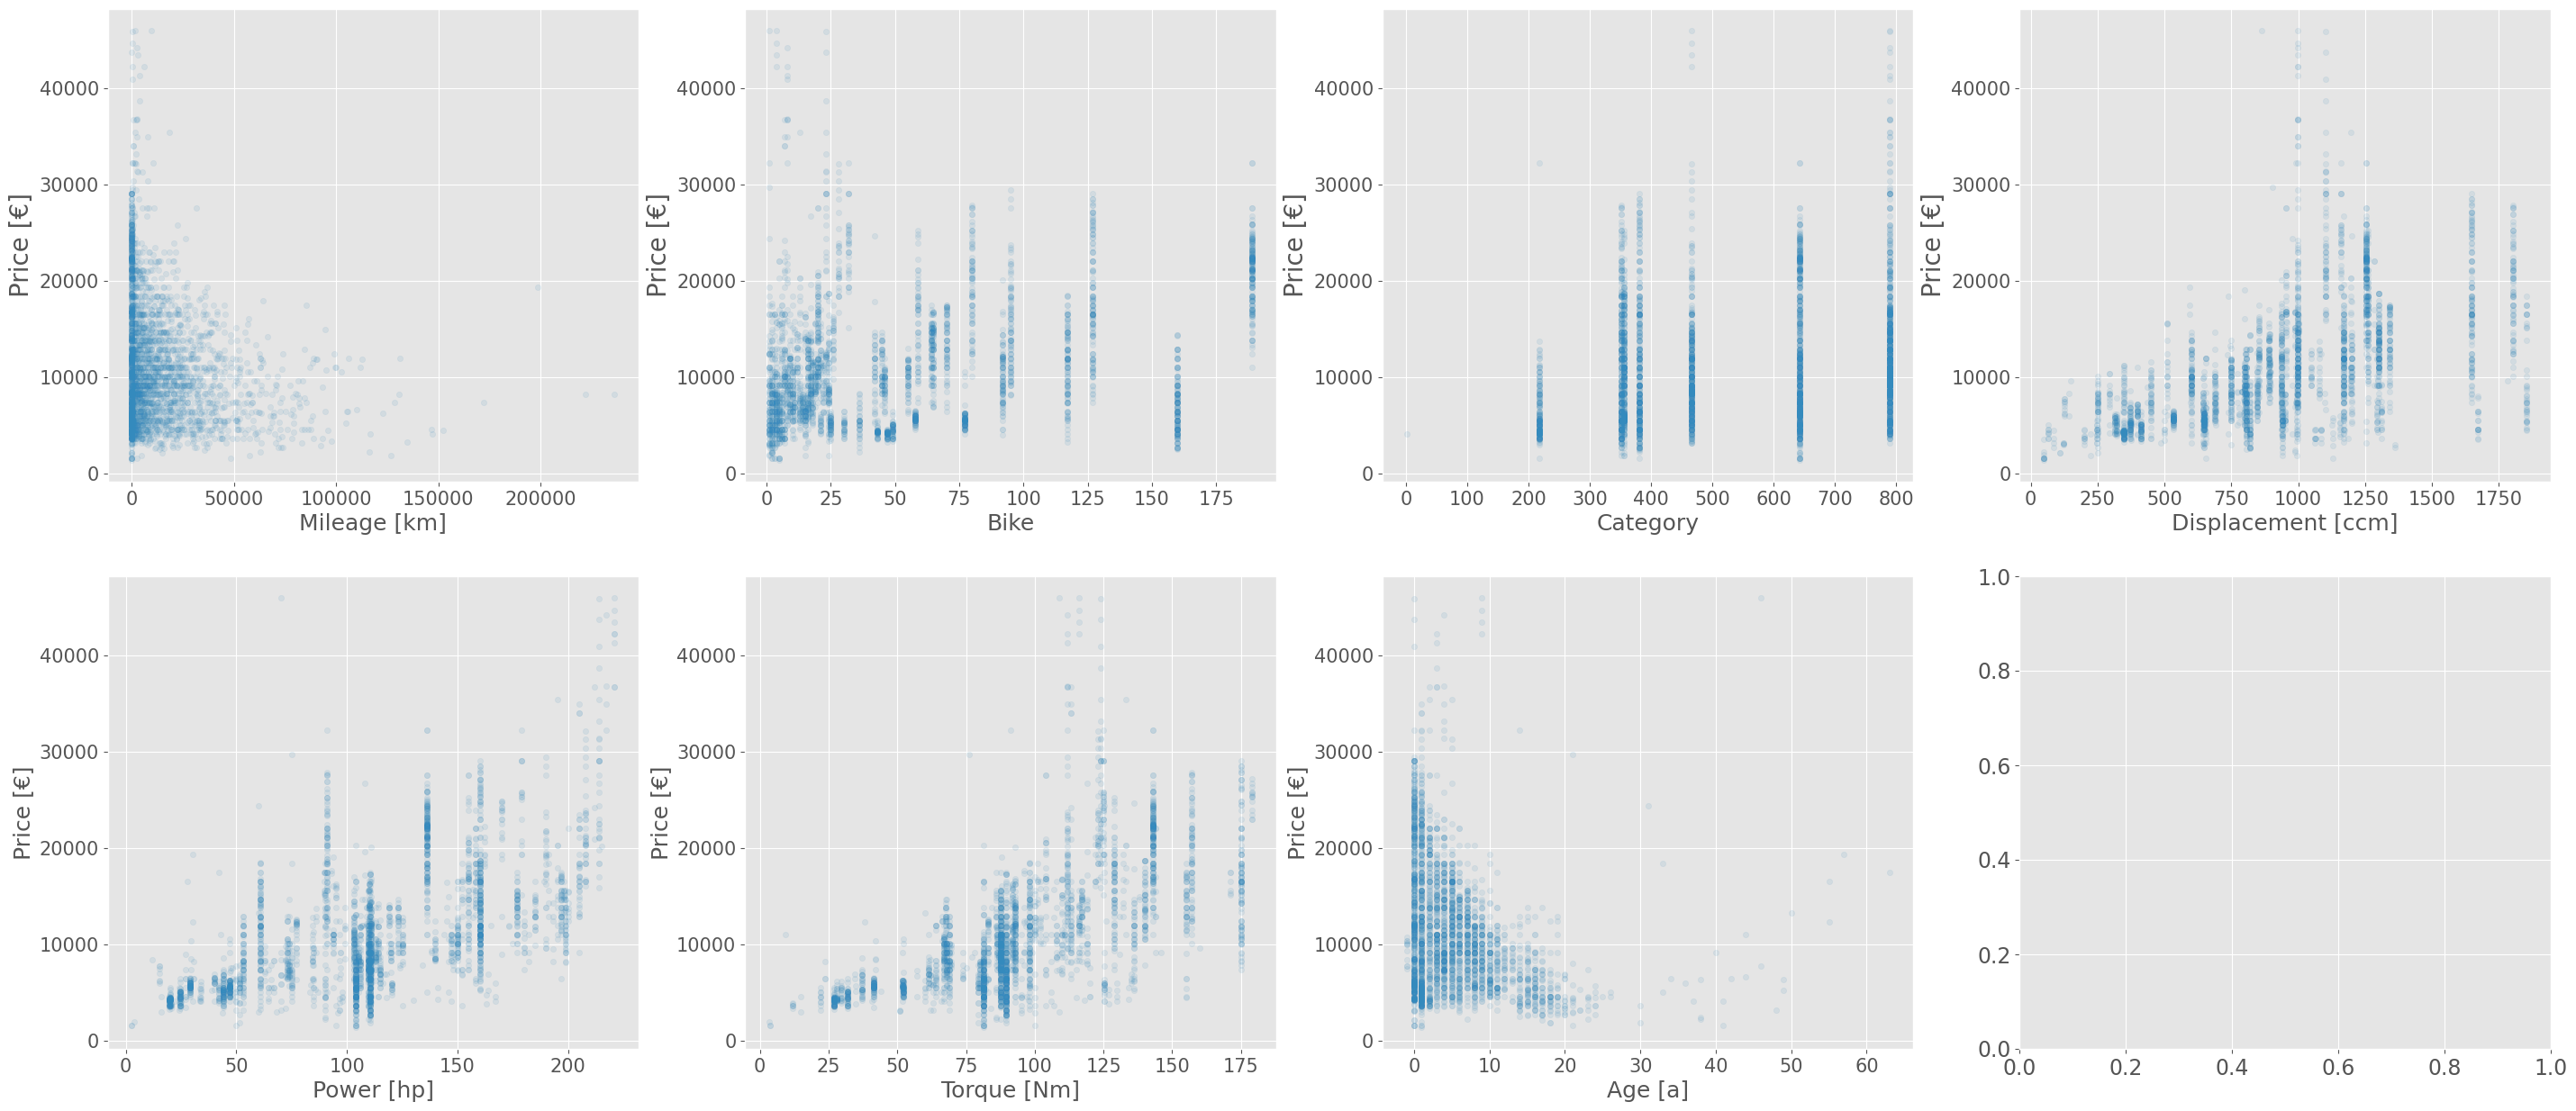
\includegraphics[width=1.25\textwidth]{"content/pics/Price_Attribute_Scatter.png"}}
        \caption{Scatter plots of the training attributes with the target value (\textit{Price [€]}).}
        \label{fig:Scatterplot_Price}
\end{figure}
\\When handling big datasets, a high amount of attributes while also having a very high amount of data entries can lead
to long training times, overtraining and long waiting times for hyperparameter optimisation. Hence, one wants to look at the correlation
of different used attributes. The correlation matrix for the used numerical variables is shown in \autoref{fig:Corr_matrix}.
\begin{figure}[!]
    \centering
        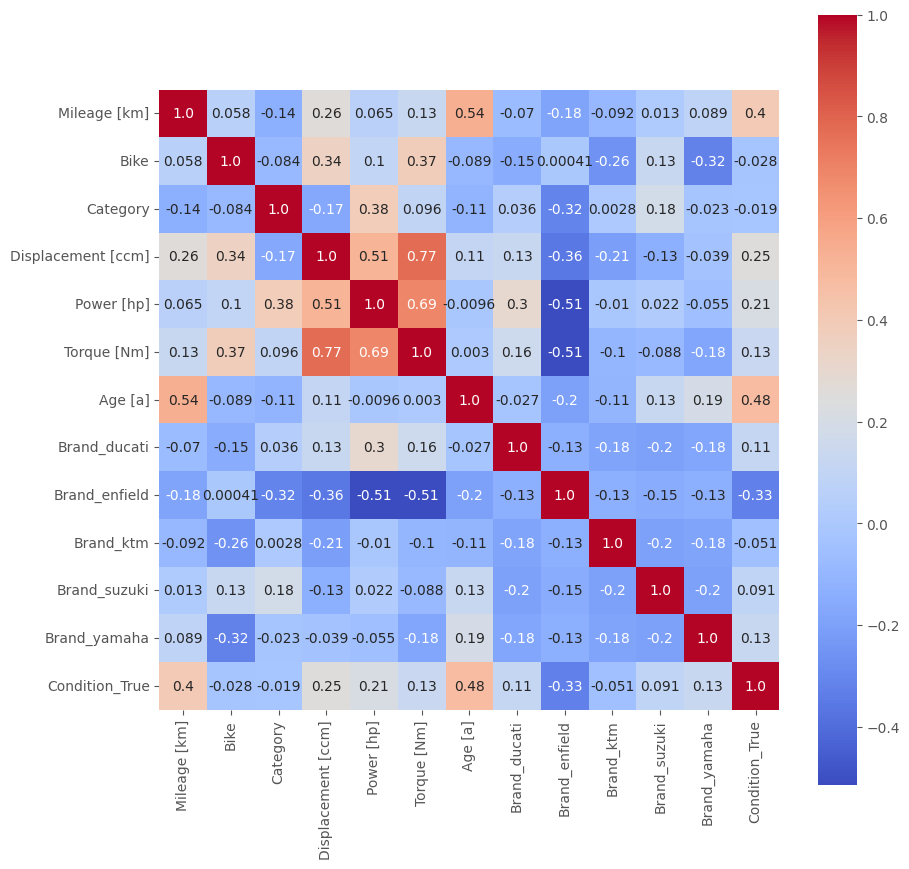
\includegraphics[width=0.8\textwidth]{"content/pics/correlation_matrix.png"}
        \caption{Correlation matrix of the provided dataset attributes.}
        \label{fig:Corr_matrix}
\end{figure}
\\Some attributes like the torque, power and displacement show high correlation, which is expected to to their mechanical origin.
Also, the mileage and age, as well as the brand \textit{Royal Enfield} and the engine specifics are highly correlated. However,
no variables will be discarded at this step, due to the already low number of attributes and the later performed feature selection.\\
Another useful method is to look at the behaviour of the data after different scaling are applied. As for the provided attributes,
the different scaling methods are observed for the \textit{Mileage} and \textit{Age} attribute. As they have the most fluent distributions
and nice correlations with the price. The scatter plots of these two attributes for \textit{Standard}, \textit{Robust}, \textit{Gaussian},
\textit{Min-Max}, \textit{Max-Abs} and \textit{Uniform} scaling are shown in \autoref{fig:Scaling}. The scalers have been used from 
the \textbf{sklearn.preprocessing}\cite{sklearn_preprocessing} library. The online documentations offers more insides on the type of scaling.
In the training of the single models, the standard, robust and normalised scaling are compared with no scaling in more detail.
\begin{figure}
    \centering
    \begin{subfigure}[b]{0.48\textwidth}
        \centering
        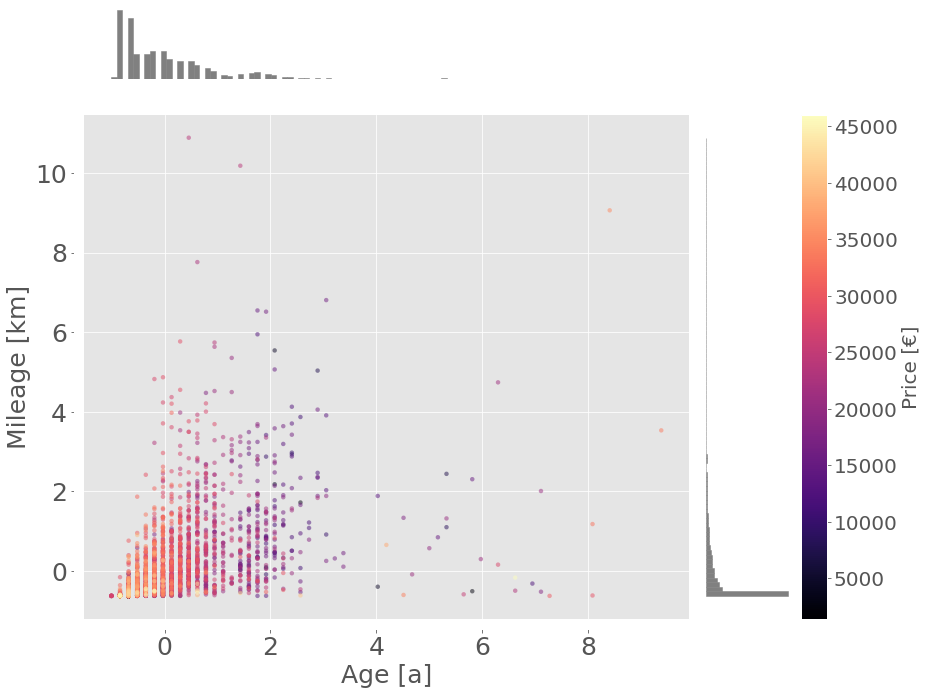
\includegraphics[width=\textwidth]{"content/pics/Scatter_Standard.png"}
        \caption{Standard Scaling.}
    \end{subfigure}
    \hfill
    \begin{subfigure}[b]{0.48\textwidth}
        \centering
        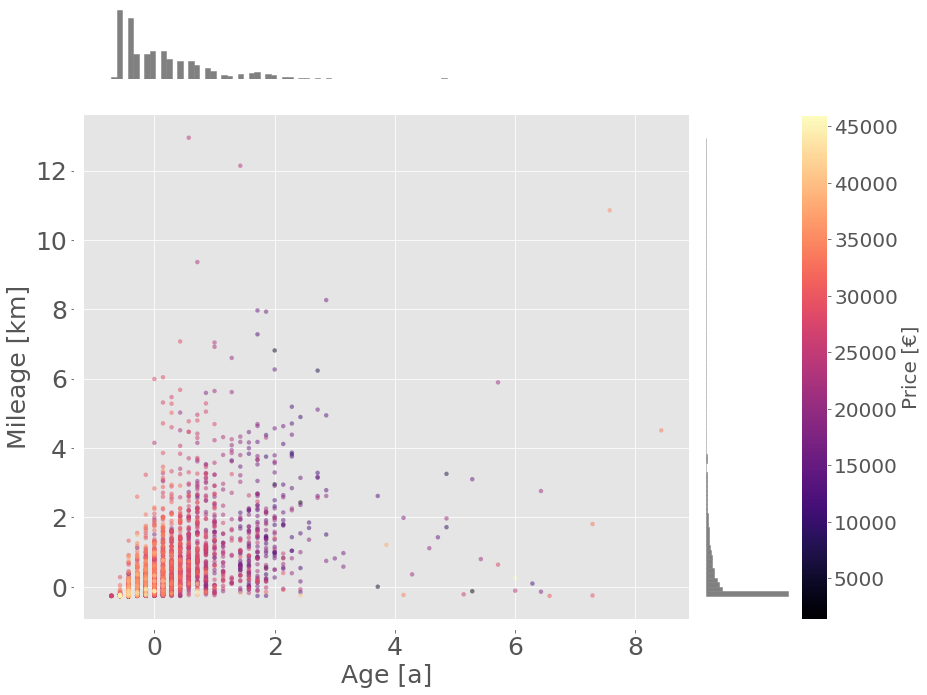
\includegraphics[width=\textwidth]{"content/pics/Scatter_Robust.png"}
        \caption{Robust Scaling.}
    \end{subfigure}
    \vfill 
    \begin{subfigure}[b]{0.48\textwidth}
        \centering
        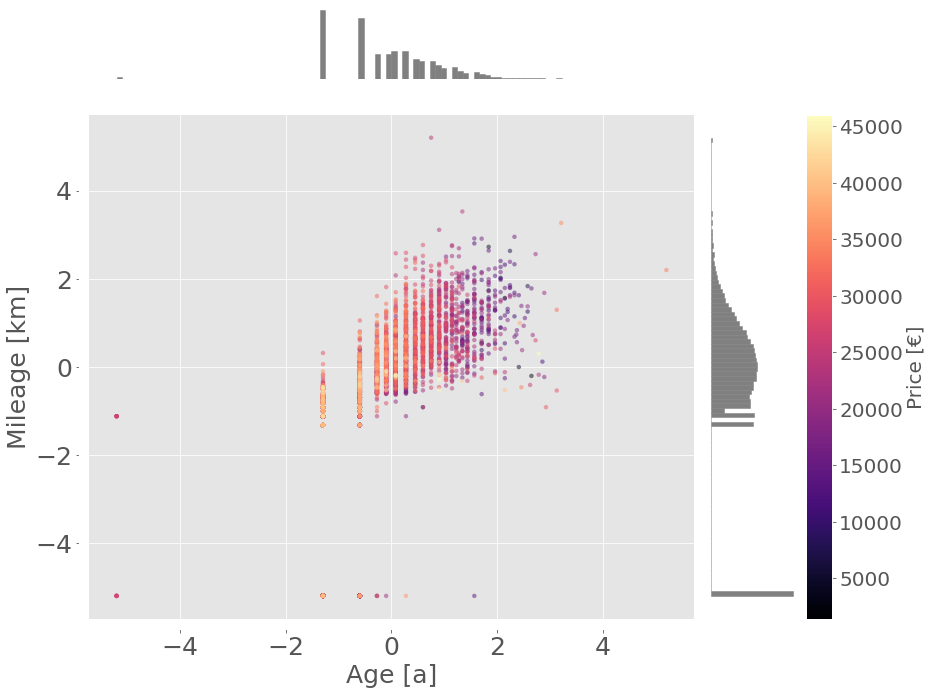
\includegraphics[width=\textwidth]{"content/pics/Scatter_Normal.png"}
        \caption{Gaussian Scaling.}
    \end{subfigure}
    \hfill
    \begin{subfigure}[b]{0.48\textwidth}
        \centering
        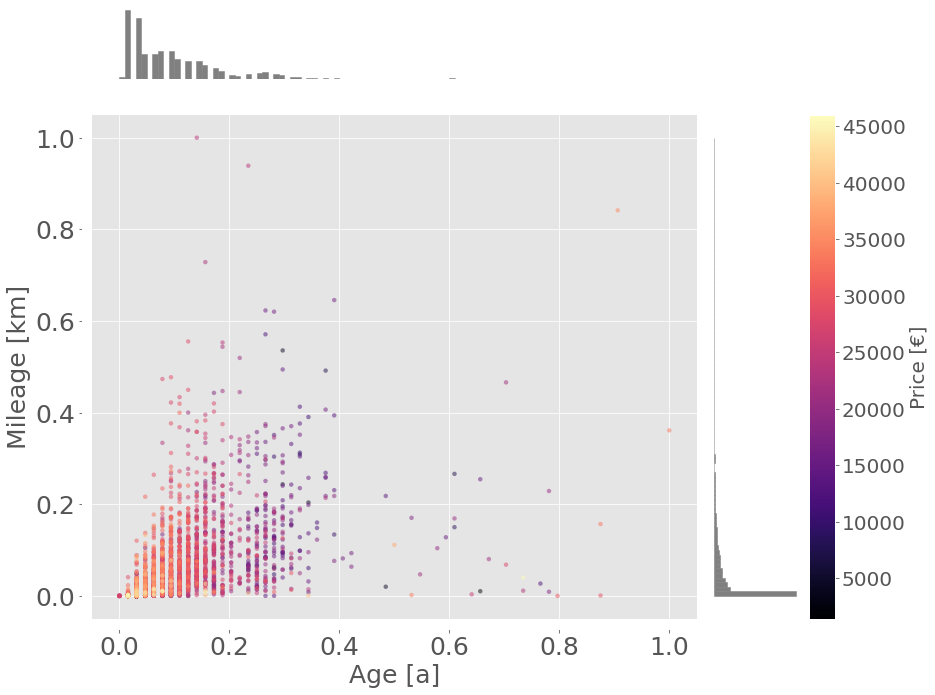
\includegraphics[width=\textwidth]{"content/pics/Scatter_MinMax.png"}
        \caption{Min-Max Scaling.}
    \end{subfigure}
    \vfill 
    \begin{subfigure}[b]{0.48\textwidth}
        \centering
        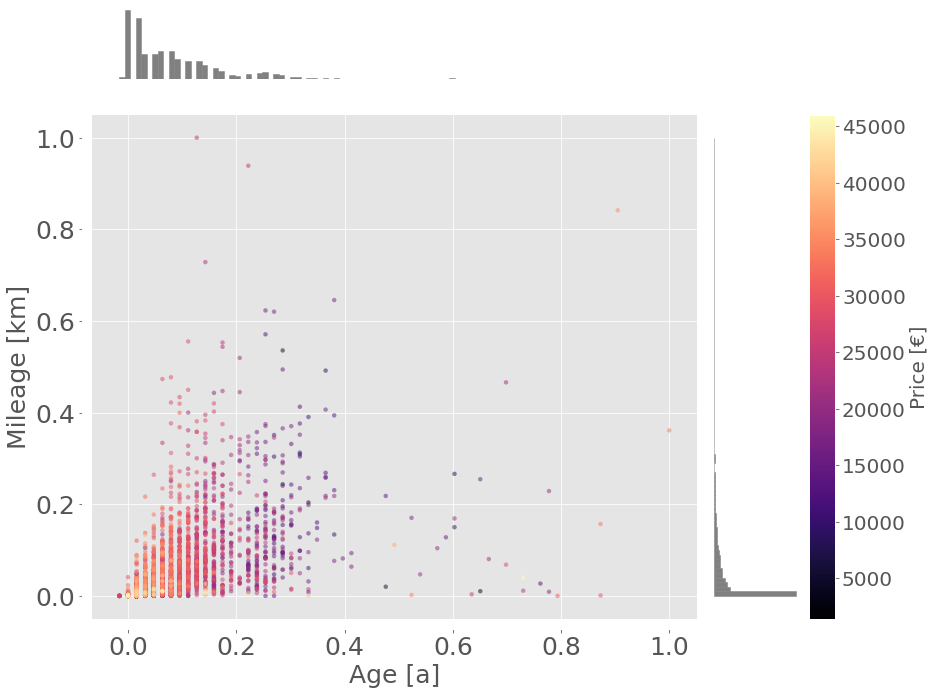
\includegraphics[width=\textwidth]{"content/pics/Scatter_MaxAbs.png"}
        \caption{Max-Abs Scaling.}
    \end{subfigure}
    \hfill
    \begin{subfigure}[b]{0.48\textwidth}
        \centering
        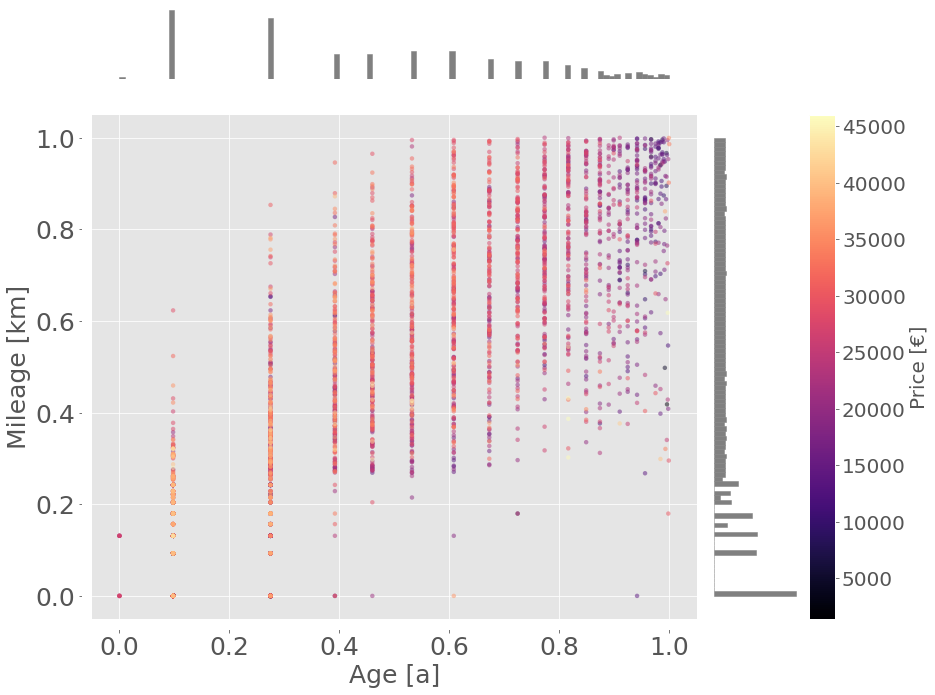
\includegraphics[width=\textwidth]{"content/pics/Scatter_Uniform.png"}
        \caption{Uniform Scaling.}
    \end{subfigure}
    \caption{Scatter plot of \textit{Mileage} and \textit{Age} with different scaling methods.}
    \label{fig:Scaling}
\end{figure}
